\Chapter{Le code MAGNIS (MAGnetized Negative Ion Source)}
\chaptermark{Modèles plasmas froids magnétisés}
Dans ce chapitre, nous proposons un nouveau modèle fluide pour décrire le
transport magnétisé dans les plasmas froids. Nous discutons tout d'abord de
l'approche standard de modélisation des plasmas froids, des problématiques qui
lui sont propres ainsi que des difficultés rencontrées lors du développement du
modèle basé sur les vitesses de dérive. La suite concerne l'élaboration du
nouveau modèle, nous le dérivons en expliquant les différents
termes essentiels à description du transport dans les plasmas froids puis nous
détaillons le schéma numérique original utilisé pour résoudre le modèle.
\section{Problématique}
La plupart des modèles fluides décrivant les phénomènes de transport
magnétisés dans les plasmas froids sont basés sur les équations de
dérive-diffusion (chapitre \ref{derivediffusion}). Cependant, au delà d'une
certaine intensité de champ magnétique, l'anisotropie du transport rend la résolution
numérique de ces équations complexe voire impossible\footnote{Le problème est alors
généralement adressé à travers le développement de
modèles cinétiques numériquement très coûteux, et nécessitant à priori la
résolution d'échelles de l'ordre de la longueur de Debye et de la fréquence plasma.}. 
Celles-ci sont en fait peu adaptées au transport fortement magnétisé. 


Un indice nous est donné en considérant la
description du transport transverse par les vitesses de dérive (cf.
introduction) où l'équilibre des courants fait intervenir la divergence de
la dérive de polarisation. Cette dérive, essentielle dans la dynamique du transport 
transverse, est absente du modèle qui néglige totalement l'inertie des particules. Le modèle de
dérive-diffusion cherche une solution stationnaire à un problème intrinsèquement non-stationnaire.

D'un autre côté, 

\section{Description du modèle}
Le plasma est constitué d'électrons et d'une ou plusieurs espèces d'ions
de charge $q_s$ et de masse $m_s$. On considère un plasma de taille $L$, 
confiné et en interaction avec des parois à travers une gaine
large de quelques longueurs de Debye. La longueur $L$ est prise suffisement 
grande $\lambda_D\ll L$ pour supposer le plasma quasi-neutre. Le champ magnétique $\mathbf{B}$ imposé
est de plus stationnaire, de sorte que le champ électrique dérive directement d'un potentiel électrostatique
$\mathbf{E}=-\nabla U$. Le transport est décrit dans le plan perpendiculaire au champ magnétique et tient compte
des pertes à la paroi en les intégrant le long de la direction parallèle. 
\subsection{Equations de conservation}
Comme discuté en introduction, nous retenons tous les termes de l'équation du moment :
\begin{equation}
	\partial_t \mathbf{u}_s + \mathbf{u}_s\cdot\nabla\mathbf{u}_s+\nu_s\mathbf{u}_s+\omega_s\mathbf{b}\times\mathbf{u}_s=-\frac{q_s}{m_s}\left(\nabla U+\frac{\nabla p_s}{q_sn_s}\right)
\end{equation}

où $n_s$ est la densité de l'espèce considérée, $\mathbf{u}_s$ sa vitesse fluide, $p_s$ la pression, $U$ le potentiel électrostatique,
$\omega_s=q_sB/m_s$ la fréquence cyclotronique et $\nu_s$ la fréquence de collision effective.
Le transfert de quantité de mouvement dû aux collisions contient la perte liée à l'ionization $\nu_s=\nu_{s}^{iz}+\nu_{s}^{sn}+\nu_{s}^{ie}$
où $\nu_{s}^{sn}$ et $\nu_{s}^{ei}$ sont respectivement les fréquences de collisions particules chargées - neutres et de collisions Coulombienne.

L'évolution de chaque espèce est décrite par une équation de continuité :
\begin{equation}
	\partial_t n_s + \nabla\cdot\left(n_s\mathbf{u}_s\right)=S_s(T_e)
\end{equation}

avec $S_s$ un terme d'ionisation, fortement dépendant de 
la température électronique $T_e$. En considérant l'hypothèse de quasi-neutralité, la somme des équations de continuité 
conduit à l'équation de conservation du courant :
\begin{equation}
	\label{eqCourant}
	\nabla\cdot(\sum_sq_sn_s\mathbf{u}_s)=0
\end{equation}

Eq. \ref{eqCourant} couple les différentes espèces en contrôlant l'évolution du potentiel électrostatique $U$.
L'équation de conservation de l'énergie est obtenue classiquement en substituant l'équation de continuité 
afin d'éliminer le terme convectif :
\begin{equation}\begin{split}
\frac{3}{2}n_e\partial_tT_e + \nabla\cdot(\mathbf{Q}) + \left(\frac{5}{2}S_e-\partial_tn_e\right)T_e
\\=n_e\mathbf{u}_e\cdot\left(\nabla U-\frac{5}{2}\nabla T_e\right)-n_e\left(P_{ext}-\Pi\right)
\end{split}
\end{equation}

où $S_e$ est le terme source d'électrons lié à l'ionisation, $P_{ext}$ la puissance extérieure déposée dans le plasma
 et $\Pi$ le terme de perte d'énergie dû aux collisions. La fermeture du modèle se fait alors sur le flux de chaleur $\mathbf{Q}$ 
 \cite{Golant} :
\begin{equation}
	\partial_t \mathbf{Q} + \nu_e\mathbf{Q}+\omega_e\mathbf{Q}\times\mathbf{b} = -\frac{5}{2}\frac{e^2}{m_e}n_eT_e\nabla T_e
\end{equation}

Le flux de chaleur est magnétisé de la même façon que le flux de matière et dépend principalement 
du gradient de température. Dans les sources magnétisées, où la longueur de gradient thermique est de 
l'ordre de grandeur de la largueur du filtre magnétique, le flux de chaleur influence fortement le transport
transverse. Il doit donc nécessairement être pris en compte et décrit là encore avec le minimum d'approximations.
 
\subsection{Conditions aux limites}
Le modèle est complété par la définition de conditions aux limites intégrant le maximum de 
considérations physiques. Dans le cas d'une paroi conductrice, un modèle classique de gaine est utilisé. Les 
flux ioniques et le flux électronique sont alors définis en l'entrée de gaine par : 
\begin{align}
	\boldsymbol{\Gamma}_i\cdot\mathbf{n}&=n.\max\left(c_s,\mathbf{u_i}\cdot\mathbf{n}\right)=n.\max\left(\left(\frac{eT_e}{m_i}\right)^{\text{\textonehalf}},\mathbf{u_i}\cdot\mathbf{n}\right)
	\\
	\boldsymbol{\Gamma}_e\cdot\mathbf{n}&=n.v_{th}=n\left(\frac{eT_e}{2\pi m_e}\right)^{\text{\textonehalf}}\exp\left({-\frac{\Phi-\Phi_w}{T_e}}\right)
\end{align}

où $\mathbf{n}$ est le vecteur normal à la paroi. Les ions sont perdus au minimum avec la vitesse acoustique, 
mais éventuellement avec une vitesse supersonique. La condition limite pour le courant est par conséquence définie 
par :
\begin{equation}
	\mathbf{j}\cdot\mathbf{n}=\left(\sum_s\boldsymbol{\Gamma}_s-\boldsymbol{\Gamma}_e\right)\cdot\mathbf{n}
\end{equation}

Dans le cas d'une paroi isolante, la surface se polarise pour assurer la nullité du courant sortant :
\begin{equation}\begin{split}
	\mathbf{j}\cdot\mathbf{n}=0\Leftrightarrow
	\Phi_w=\Phi-T_e.ln\left(\left(\frac{2\pi m_e}{eT_e}\right)^{\text{\textonehalf}}\frac{1}{n_e}\sum_s \boldsymbol{\Gamma}_s\right)
\end{split}\end{equation}

Pour le flux d'énergie, 
\begin{equation}
	\frac{5}{2}n_eT_e\mathbf{u}_e\cdot\mathbf{n}+\mathbf{Q}\cdot\mathbf{n}=
	n\left(\frac{eT_e}{2\pi m_e}\right)^{\text{\textonehalf}}\exp\left({-\frac{\Phi-\Phi_w}{T_e}}\right)\left(2T_e+\Phi-\Phi_w\right)
\end{equation}

\begin{equation}
	\mathbf{Q}\cdot\mathbf{n}=n\left(\frac{eT_e}{2\pi m_e}\right)^{\text{\textonehalf}}\exp\left({-\frac{\Phi-\Phi_w}{T_e}}\right)\left(\Phi-\Phi_w-\frac{1}{2}T_e\right)
\end{equation}


\section{Implémentation numérique du modèle}
\subsection{Discrétisation temporelle}
\subsection{Discrétisation spatiale}
\begin{figure}[htbp]
	\centering
	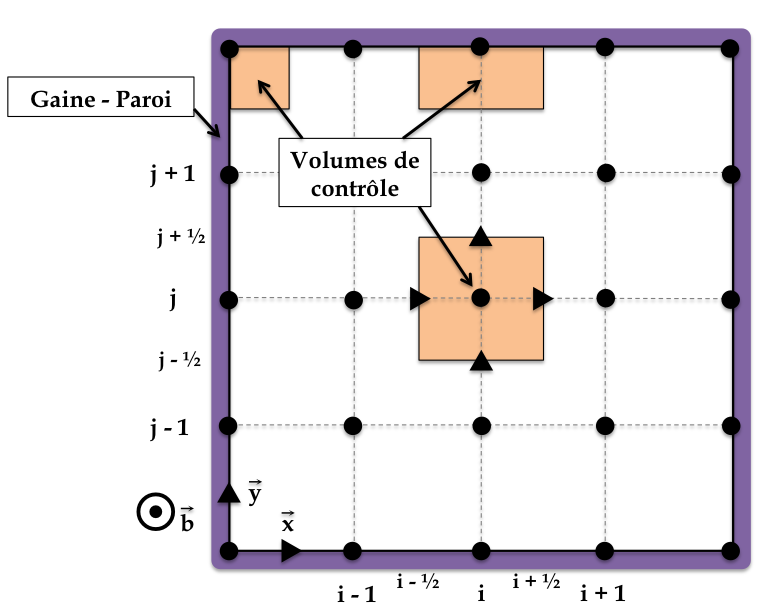
\includegraphics[height=64mm,width=80mm]{figures/grid.png}
	{\caption{Maillage 2D pour les schémas volumes finis}
	\label{maillage}}
\end{figure}
\begin{equation}
	S_s(T_e)=n_en_gk_{s}^{iz}(T_e)
\end{equation}
où $n_g$ est la densité du gaz et $k_{s}^{iz}$ le coefficient d'ionisation spécifique à l'espèce. 


\section{Vérification et validation}
\subsection{Convergence en temps et en espace}
\subsection{Influence du champ magnétique}
\subsection{Réponses à la température}


